\section{Database}

Med udgangspunkt i \gls{moscow} analysen i afsnit~\pageref{sec:moscow} blev det første udkast til databasen lavet. Meningen var at opfylde punktet: 

\begin{itemize}
	\item Der skal kunne oprettes en bruger til systemet.
\end{itemize}

For at lave dette på en måde som gjorde udvidelse let, kom første udkast til at se ud som vist på figur~\ref{fig:database_class_1}. Adgangen til databasen skulle være simpel. Dette var på grund af grænsefladen til resten af system, som skulle udvikles samtidigt. På denne måde skulle de øvrige grupper ikke ændre deres brug af \textit{ISmartpool} interfacet.  skulle der laves én klasse som ville have associationer til specialiserede klasser. Figur~\ref{fig:database_class_1} viser hvordan kaldet fra \textit{context} går gennem klassen \textit{ISmartpool}

\begin{figure}[h]
	\centering
	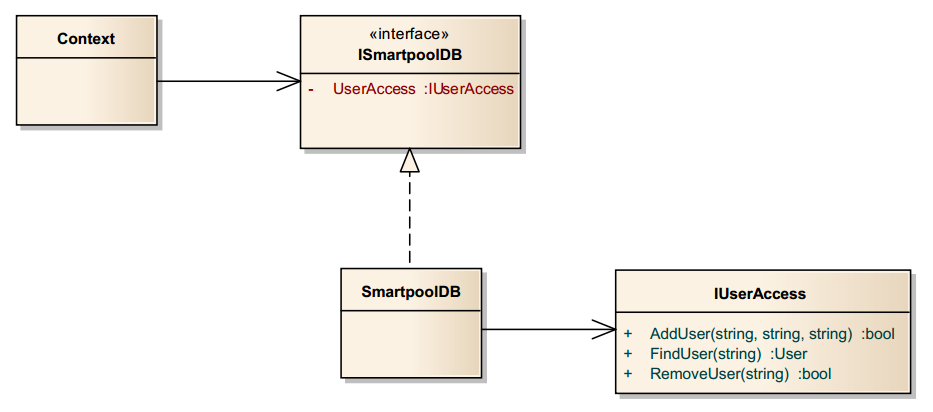
\includegraphics[width=0.9\linewidth]{figs/design/database_class_1}
	\caption{Første design for database-adgang.}
	\label{fig:database_class_1}
\end{figure}

På denne måde skulle \textit{UserAccess} klasse så stå for adgang til brugerinformationer i databasen. 

Der skulle så laves en simple database, med det eneste formål at kunne indeholde disse basale informationer om brugerne af systemet.

\begin{itemize}
	\item Navn (for, mellem og -efternavn)
	\item Email
	\item Kodeord
\end{itemize}

Med \gls{ef} blev følgende model lavet til at opfylde dette krav.

\begin{figure}[h]
	\centering
	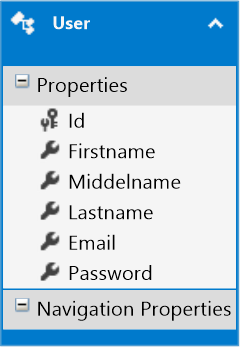
\includegraphics[width=0.25\linewidth]{figs/design/database_model_1}
	\caption{Model for første design for database-adgang.}
	\label{fig:database_model_1}
\end{figure}

Udfra dette blev et script genereret, som så skulle køres mod en localdb. Nu var databasen oprettet og implementeringen af \textit{UserAccess} kunne starte.

\subsection{Persistering af sensordata}
%Husk at tage udgangspunkt historisk pool data US
Da Smartpool systemet kræver lagring af større mængder data er der gjort en del overvejelser på området. En tidlig udgave af database designet kan ses på \ref{fig:databaseERD_final_uml}. Her gemmes alt indsamlet data i én stor tabel. Dette er uhensigtsmæssigt i forbindelse med data queries, og designet er siden blevet optimeret. Ser man på \ref{fig:databaseERD_final_uml}, er entiteten MonitorUnit blevet fjernet helt. Dataen ligger her i hver sin respektive tabel med henblik på type. Der er tilføjet en Data entitet der har et timestamp som attribut. Man kan derved finde tidsspecfik data, blot ved at kende den Data entitet der videre kender til brugerens pool. På denne måde er søgetiden optimeret med en faktor 4. Dog vil søgetider stadig blive længere jo flere pools der tilføjes i systemet.

\subsubsection{Fremtidigt arbejde}
En videre optimering må være at oprette nye data tabeller hver gang der oprettes en pool i systemet. Dette vil mindske søgetider drastisk. Envidere kan data der er ældre end x antal dage, flyttes til en anden tabel. På denne måde vil der komme et maximum for søgetider i nyere data.

\begin{figure}
	\centering
	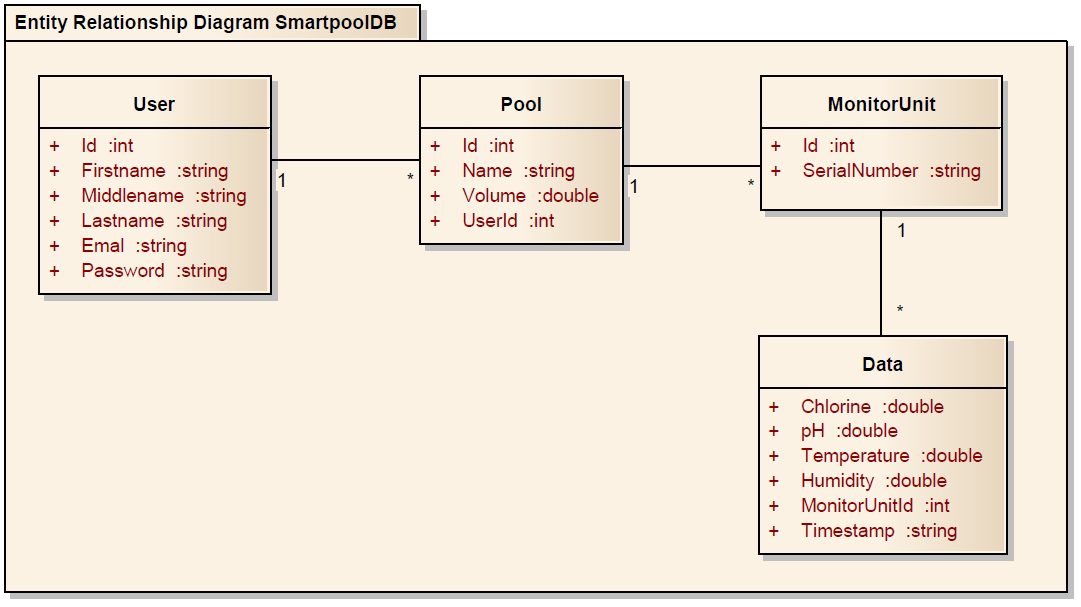
\includegraphics[width=\linewidth]{figs/design/databaseERD_old_uml}
	\caption{Første udgave af ER diagram, UML notation}
	\label{fig:databaseERD_old_uml}
\end{figure}

Sensor data persisteres i hver sin tabel.

\subsection{Endeligt database design}

\begin{figure}
\centering
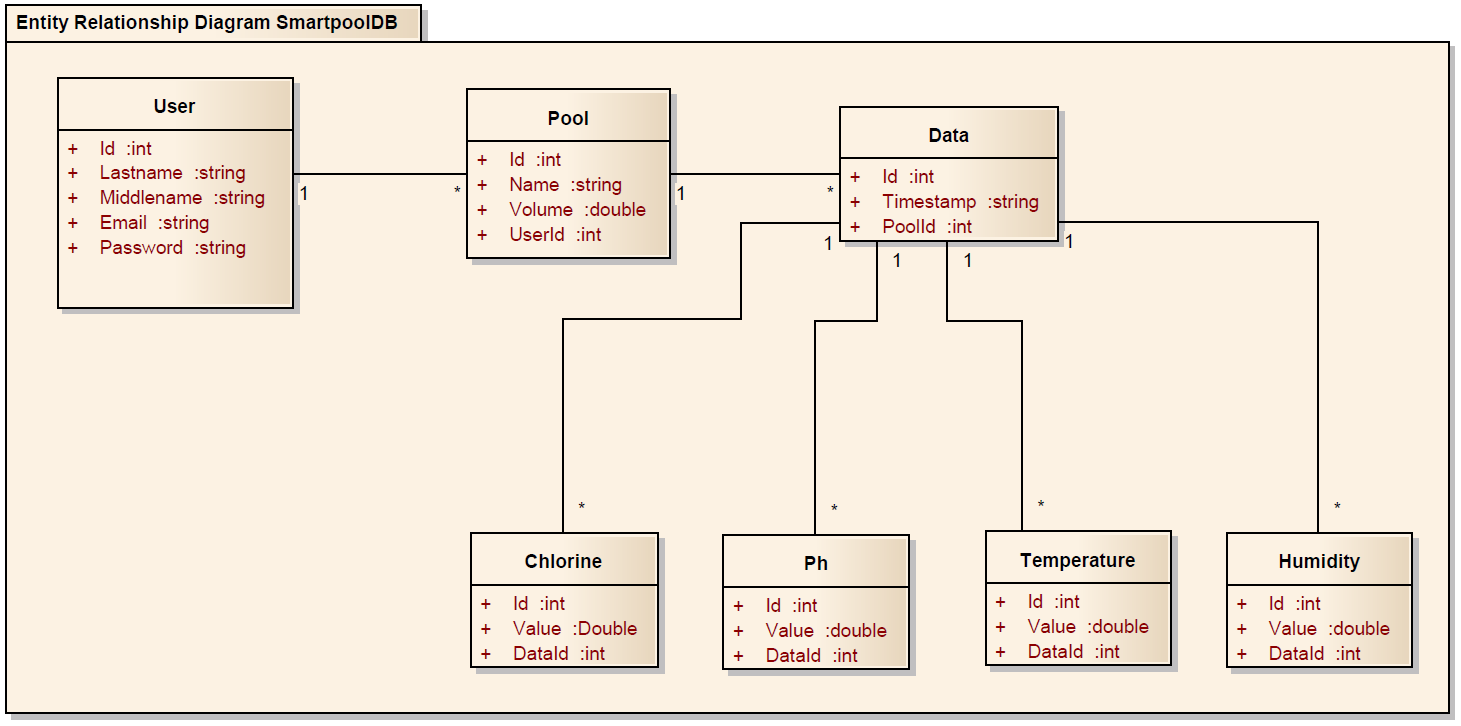
\includegraphics[width=\linewidth]{figs/design/databaseERD_final_uml}
\caption{Endeligt ER diagram, UML notation}
\label{fig:databaseERD_final_uml}
\end{figure}




